% Data flow diagram
% Author: David Fokkema
\documentclass{article}
\usepackage{tikz}
\usetikzlibrary{shapes,arrows}
\usepackage{pdflscape}
\usepackage[papersize={6.8cm, 3.2cm}, text={6.8cm, 3.4cm}]{geometry}
\usetikzlibrary{decorations.text}
\usepackage{xcolor}
% \selectcolormodel{gray}

\begin{document}
\thispagestyle{empty}
%\begin{landscape}
\begin{center}
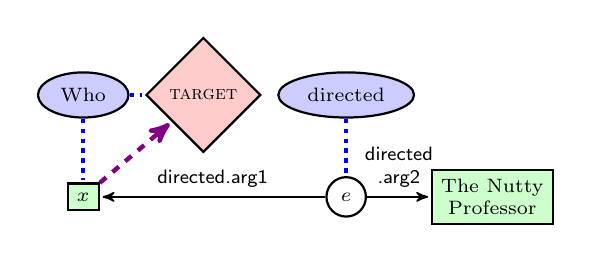
\begin{tikzpicture}[
  font=\sffamily,
  every matrix/.style={ampersand replacement=\&,column sep=0.2cm,row
sep=0.2cm,font=\scriptsize},
  entity/.style={draw,thick,rectangle,fill=green!20},
  word/.style={draw,thick,ellipse,fill=blue!20},
  mediator/.style={draw,thick,circle},
  entityType/.style={draw,thick,rounded corners,fill=yellow!20,inner sep=.3cm},
  mathType/.style={draw,thick,diamond,fill=red!20,font=\sc\scriptsize},
  mediatorToEntity/.style={->,>=stealth',shorten
>=1pt,semithick,black,sloped,above,font=\sffamily\scriptsize},
  typeToEntity/.style={->,>=stealth',shorten
>=1pt,semithick,black,sloped,above,font=\sffamily\scriptsize},
  wordToEntity/.style={-,>=stealth',shorten >=1pt,ultra
thick,dotted,blue,sloped,above,font=\sffamily\scriptsize},
  entityToMath/.style={->,>=stealth',shorten >=1pt,ultra
thick,dashed,violet,sloped,above,font=\sffamily\scriptsize},
  every node/.style={align=center}]

  % Who is the director of The Nutty Professor
  
  % Position the nodes using a matrix layout
  \matrix{ 
   \node[word] (wWho) {Who}; \&  \node[mathType] (mQues) {target}; \& \node[word] (wDirected)
{directed}; \&  \\
    \node[entity] (eWho) {$x$}; \& \& \node[mediator] (mDirector) {$e$}; \& \node[entity]
(eNutty) {The Nutty\\Professor};
\\
   % \node[entityType] (tDirector) {director}; \& \node[word] (wDirector) {director$_4$}; \\
  };
 
  % words to entities
  \draw [wordToEntity] (wWho) edge node {}  (eWho);
  % \draw [wordToEntity] (wNutty) edge node {}  (eNutty);
  \draw [wordToEntity] (wDirected) edge node {}  (mDirector);
  
  % words to types
  % \draw [wordToEntity] (wDirector) edge node {}  (tDirector);
  
  % type to entity
  % \draw [typeToEntity] (tDirector) edge node {type}  (eWho);
  
  % event word to mediators
  % \draw [wordToEntity] (wDirector) edge node {}  (mDirector);
  
  % mediator to entities
  \draw [mediatorToEntity] (mDirector) edge node {directed.arg1}  (eWho);
  \draw [mediatorToEntity] (mDirector) edge node {directed\\.arg2} 
(eNutty);
   
   \draw [entityToMath] (eWho) edge node {}  (mQues);
   \draw [wordToEntity] (wWho) edge node {}  (mQues);
  
\end{tikzpicture} 
\scriptsize $\textsc{target}(x) \wedge \mbox{directed.arg1}(e, x) \wedge \mbox{directed.arg2}(e,
\mathrm{The Nutty Professor})$
\end{center}


\end{document}
